\section{Question 2: Navigation}

This exercise required that the robot arm navigate around an obstacle to reach an endpoint, from a start point. By describing the space around the robot arm with a matrix (alpha x beta) of a 5\% resolution (i.e. the resolution of our grid was divided by a factor of 5 to increase speed at the consequence of accuracy, we were able to assign rewards and penalties to the endpoint and the obstacle(s)/boundaries of the space respectively. One of the first problems we encountered was in our code. When implemented, the robot arm seemed to move only partially to its destination. A visualization of the matrix showed that the reward set at some point (alpha, beta) was only propagating to points in the beta direction but not the alpha direction. This was found to be a technical problem where the iterations of the policy in the alpha direction (up/down) were not based on the calculations of the value function but instead based on values equal to zero due to the resetting of the loop. Further complications occurred with the setting of certain constants such as the resolution of the space, reward/punishment values and the discount factor of our value function. We discovered a difficulty between the two motors of the robot arm, being that if the second portion of the arm couldn’t move towards the reward destination without intersecting with the punishment region of the space, it would get caught in a loop in the policy instead of the first portion of the arm adjusting to allow the space required. We overcame this issue with a couple methods. The first was effective but it relied on increasing the speed of the motors and sampling time of the position of the arms. This lead to consistent overshooting of the obstacle and problematic space mentioned previously but ultimately resulted in constant overshooting of the final destination. The second and more successful method was to fine tune a number of the parameters including increasing the punishment of the obstacle and the reward of the destination, increasing the discount factor to enhance immediate reward than later reward and decreasing the resolution to add noise to the space.
The following graphs show the occupied space and the path the robot arm took to reach the desired location. The desired location was a hard coded value that was arbitrary set and the starting location was a random point that the arm was left at. The program would have some difficulty when there was a limited range of motion without interception with the block as demonstrated around angle 5,0. 

\begin{figure}[tbd]
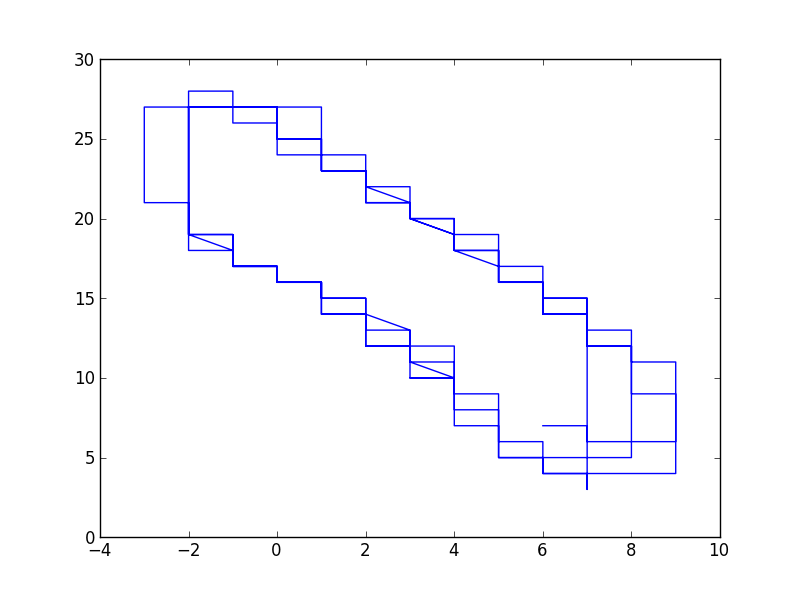
\includegraphics[width=0.5\textwidth]{images/image.png}
\caption{\label{occupied} Objects outline in space grid map}
\end{figure}

\begin{figure}[tbd]
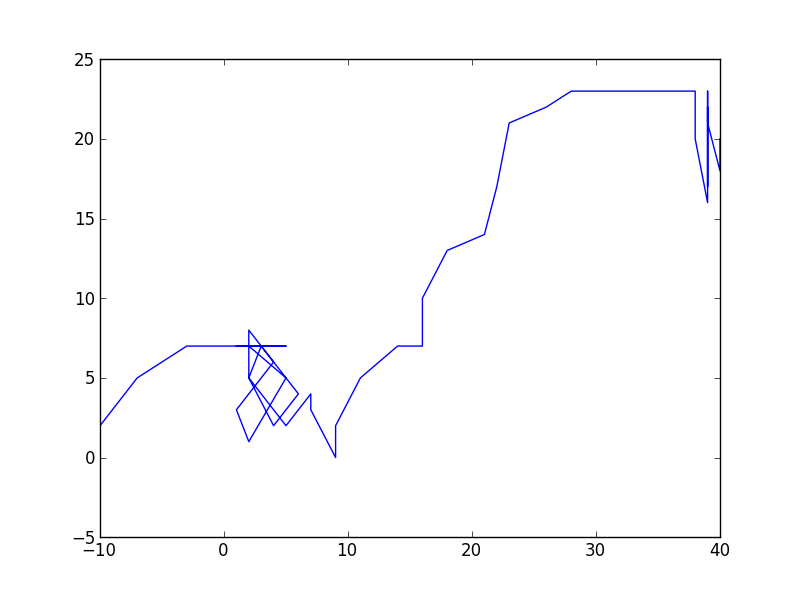
\includegraphics[width=0.5\textwidth]{images/image2.png}
\caption{\label{path} Path of Robot Arm to get to desired location}
\end{figure}